\documentclass[12pt]{article}
\usepackage[utf8]{inputenc}
\usepackage{hyperref}
\usepackage{graphicx}
\graphicspath{ {img/} }
\usepackage[justification = centering]{caption}
\usepackage{float}
\usepackage{amsmath}
%\usepackage[version=4]{mhchem}
\usepackage{booktabs} % nice rules (thick lines) for tables
\usepackage{microtype} % improves typography for PDF
\usepackage{float}
\usepackage{multicol}

\newcommand{\labname}{448 Group 8 Nuclear Shipping\xspace}%

%\course{NPRE 448}
\title{Nuclear-powered Shipping}
\author{Louis Kissinger, Brad Ellis, and Adam Pichman \\Course: NPRE 458; Advisor: Magdi Ragheb}
\date{February 22, 2019}
\makeatletter
\setlength{\@fptop}{0pt}
\makeatother

\begin{document}

%TITLE PAGE
\maketitle
%
\pagebreak
%ABSTRACT
\begin{abstract}
Nuclear power was analyzed as an alternative to fossil fuel combustion for propulsion of large boats. In particular, ... 
\end{abstract} 

\pagebreak
\tableofcontents

%\begin{multicols}{2

%%%%%%%%%%%%%%%%%%%%%%%%%%%%%%%%%%%%%%%%%%%%%%%%%%%%%%%%%%%%%%%%%%%%%%%%%%%%%%%%
\section{Introduction}
Introduction

If you wanna cite Alekseev put \cite{alekseev}

If you wanna cite Carlton put \cite{Carlton}

\cite{Gravina}

\cite{Han}

\cite{iaea}

If you wanna cite Hirdaris put \cite{Hirdaris}

If you wanna cite Jacobs put \cite{Jacobs}

If you wanna cite Holtec put \cite{Holtec}



%%%%%%%%%%%%%%%%%%%%%%%%%%%%%%%%%%%%%%%%%%%%%%%%%%%%%%%%%%%%%%%%%%%%%%%%%%%%%%%%
\section{Background and State of the Art}
Background and state of the art
%%%%%%%%%%%%%%%%%%%%%%%%%%%%%%%%%%%%%%%%%%%%%%%%%%%%%%%%%%%%%%%%%%%%%%%%%%%%%%%%
\section{Conceptual Design}
\subsection{Naval concept}
\subsubsection{Oceanic tug boat}
\subsubsection{Offshore power plant and coastal tug boat}
\subsection{Reactor concept}
\subsubsection{Core concept}
\subsubsection{Neutronics analysis}
The following analysis determines the enrichment required to reach $k_\infty = 1$:

\begin{align}
k_\infty &= \eta f = 1 \\
 &= \nu \frac{\sigma_f^F}{\sigma_a^F} \frac{\Sigma_a^F}{\Sigma_a} \label{e:kinfty}
\end{align}

Approximate values of these parameters are given in table \ref{t:jaea-table}.

\begin{table}[H]
\begin{center}
  \caption{Approximate values of nuclear properties germaine to equation \ref{e:kinfty}, \cite{jaea}}
  \label{t:jaea-table}
  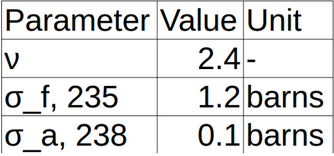
\includegraphics[width=0.5\textwidth]{full-spectrum-nuke-data}
\end{center}
\end{table}


The macroscopic cross section is by definition $\Sigma = N \sigma = \frac{\rho N_{av}}{A} \omega$. Equation \ref{e:kinfty} then reduces to:

\begin{align}
1 &= \nu \frac{^{235}\sigma_f}{^{235}\sigma_a} \frac{\frac{\omega}{235} ^{235} \sigma_a}{\frac{1 - \omega}{238} ^{238} \sigma_a} \\
 &= \nu \frac{^{235} \sigma_f}{^{238} \sigma_a} \frac{238 \omega}{235 (1 - \omega)} 
\end{align}

Upon defining a new variable $\xi = \nu \frac{^{235} \sigma_f}{^{238} \sigma_a}$, we find:

\begin{align}
\frac{1}{\xi} &= \frac{238 \omega}{235 (1 - \omega)} \\
\omega &= \frac{235}{238 \xi + 235} < 1
\end{align} 

Upon inserting the tabulated values for these cross sections, we find $\xi = 4.2$ and $\omega = 0.0336 = 3.4 \% $. The bulk of the reactor can thus be fueled without HEU.

\textbf{If the fuel is $UO_2$}, then the mass of Uranium per mass of fuel is:

\begin{align}
\frac{m_U}{m_{UO2}} &= \frac{238 (1 - \omega) + 235 \omega}{238 (1 - \omega) + 235 \omega + 32} \\
 &= 0.8817 \frac{grams}{gram} \\
n_{235} &= \omega m_u \frac{N_{av}}{235} \\
 &= 7.906 \times 10^{20}
\end{align}

If we \textbf{assume that $\frac{3}{4}$ of the fissions occur in $U_{235}$}, then the total fissile atoms per gram of fuel is $1.05 \times 10^{21}$. 

We can now determine the required mass of Uranium to produce a certain amount of energy. The core's power is related to the fission rate by a factor of 200 MeV per fission. We will \textbf{assume a core power of 1.75 GWth} for this analysis. This value roughly corresponds to 60 MWe for typical values of efficiency, which is close to the power output of the reactors we seek to imitate. The fission rate in our reactor is then $1.75 \times 10^9 \frac{Joules}{sec} \times \frac{1 MeV}{1.6 \times 10^{-13}} \times \frac{1 Fission}{200 MeV} = 5.5 \times 10^{19} \frac{fissions}{second}$.

In an \textbf{assumed 2-year refueling cycle} we would then need $5.5 \times 10^{19} \frac{fissions}{second} \times \frac{3.15 \times 10^7 s}{y} = 1.723 \times 10^{27}$ fissile atoms. 

Returning to our value of fissile atoms per gram of $UO_2$, we can find the mass of Uranium required to power our core for two years. This number is $5.5 \times 10^{19} \frac{fissions}{second} \times \frac{6.3 \times 10^7 s}{2 years} = 3.5 \times 10^{27}$

\subsubsection{Thermal analysis}
\subsubsection{Materials analysis}
\subsubsection{Alternatives}
Conceptual design
%%%%%%%%%%%%%%%%%%%%%%%%%%%%%%%%%%%%%%%%%%%%%%%%%%%%%%%%%%%%%%%%%%%%%%%%%%%%%%%%
\section{Conclusions}
Conclusions

%%%%%%%%%%%%%%%%%%%%%%%%%%%%%%%%%%%%%%%%%%%%%%%%%%%%%%%%%%%%%%%%%%%%%%%%%%%%%%%%

%%%%%%%%%%%%%%%%%%%%%%%%%%%%%%%%%%%%%%%%%%%%%%%%%%%%%%%%%%%%%%%%%%%%%%%%%%%%%%%%
\section{Acknowledgements}
Thanks to the Illinois NPRE department for their tireless work educating us. In particular, we would like to thank Professor Ragheb for his guidance and mentorship and Professor Stubbins for instructing the Senior Design course.

%%%%%%%%%%%%%%%%%%%%%%%%%%%%%%%%%%%%%%%%%%%%%%%%%%%%%%%%%%%%%%%%%%%%%%%%%%%%%%%%
\bibliographystyle{ans}
\bibliography{bibliography}
%\end{multicols}
\end{document}

